\documentclass[a4paper,12pt]{article}

\usepackage[utf8]{inputenc}
\usepackage[T1]{fontenc}
\usepackage[czech]{babel}
\usepackage{amsmath}
\usepackage{amsfonts}
\usepackage{amssymb}
\usepackage{graphicx}
\usepackage{hyperref}
\usepackage{float}
\usepackage{hyperref}

\usepackage[a4paper]{geometry}
\geometry{verbose,tmargin=2.5cm,bmargin=2cm,lmargin=2cm,rmargin=2cm}
\usepackage{fancyhdr}
\pagestyle{fancy}

% nastaven� pisma a �e�tiny
\usepackage{lmodern}
\usepackage[T1]{fontenc}
% v�cesloupcov� tabulky
\usepackage{multirow}

% vno�en� popisky obr�zk�
\usepackage{subcaption}

% automatick� konverze EPS 
\usepackage{graphicx} 
\usepackage{epstopdf}

% odkazy a z�lo�ky


% Pozn�mky p�i p�ekladu
\usepackage{xkeyval}	% Inline todonotes
\usepackage[textsize = footnotesize]{todonotes}
\presetkeys{todonotes}{inline}{}


\title{Řešení úkolu pro TurtleBot s detekcí objektů a SLAM}
\author{Michal Bouda, Erik Doležal, Ondřej Váňa}
\date{\today}

\begin{document}

\maketitle

\tableofcontents

\section{Zadání}
Úkolem práce je napsat řešení úkolu, kde má Roomba TurtleBot kopnout míč do branky označené modrými pilíři.
Rozložení problému je vidět na obrázku \eqref{fig:map}.
\begin{figure}[H]
\centering
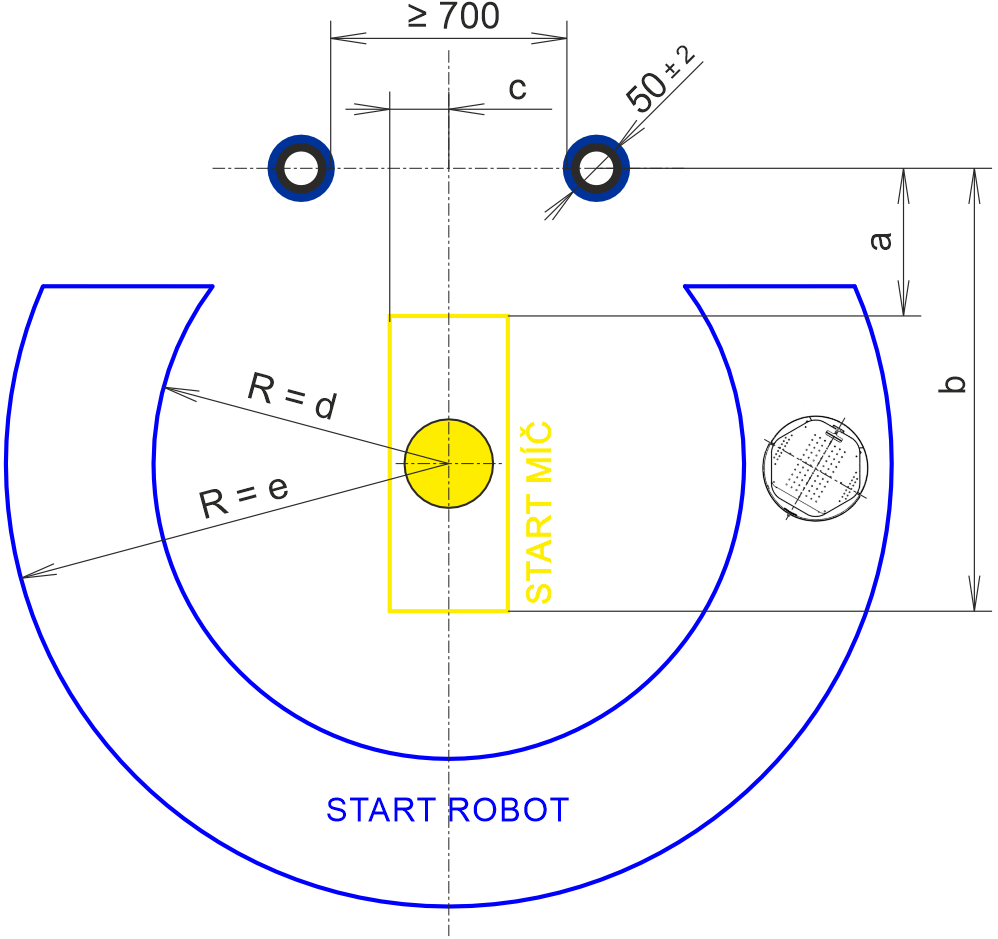
\includegraphics[width=0.4\textwidth]{pictures/map.png}
\caption{Rozložení objektů v prostoru (ze zedání)}
\label{fig:map}	
\end{figure}

\subsection{Úloha 2}
Robot má za úkol najít míč a ten kopnout mezi modré pilíře, které jsou od sebe vzdálené minimálně $700$ mm. Robot musí zastavit $20$ cm před brankou. Míč je vzdálen od osy branky maximálně $c = 150$ mm.
Míč se bude nacházet v minimální vzdálenosti $a = 500$ mm od brány a bude nejdále $b = 1,5$ m. TurtleBot bude na začátku umístěn od středu míče ve vzdálenosti $d = 0,7$ m až $e = 2,5$ m.
Za bránou může být neomezený počet pilířů.

\subsection{Úloha 3}
Od Úlohy 2 se Úloha 3 liší tím, že míč může být vzdálen od osy branky $c = 300$ mm. Vzdálenost míče od branky může být až $b = 2$ m.
Největším rozdílem je možnost výskutu až dvou překážek před čarou. Ty jsou umístěny tak, že pokaždé existuje cesta od míe k brance o minimální šířce $600$ mm.

\section{Řešení}
Naše řešení jsme rozdělili na tři hlavní části. První část je zpracování obrazu, druhá část je SLAM a třetí část je plánování a pohyb robota. Tyto části běží v hlavní smyčce programu. Naše řešení je dimenzováno pro řešení třetí úlohy. Z nedostataku času pro ošetření všech možných přídapů, jsme se ale rozhodli řešit druhou úlohu. 
Při řešení problému bylo využíváno nástroje GitHub Copilot pro jednoduché úkony pro zrychlení práce. 
\subsection{Zpracování obrazu}
Detekci objektů děláme pomocí konvoluční neuronové sítě \href{https://docs.ultralytics.com/models/}{YOLO} (You Only Look Once), kterou poté konvertujeme do \href{https://onnx.ai/}{ONNX}. Důvodem k použití CNN bylo, aby náše řešení dobře zvládalo změny v osvětlení a jiné rušivé vstupy jako například špinavý žlutý míč. Segementace obrazu pomocí barev, by mohla být v tomto ohledu nespolehlivá. Jako vstup používáme obraz z Intel RealSense D435 kamery.
\subsubsection{Trénování CNN}
YOLO model jsme museli nejdříve natrénovat na rozponávání pilířů a míče. Učinili jsme tak na více než 670 obrázcích,
které jsme pořídili pomocí kamery na robotovi. Dalších 120 jsme použili pro validaci. Obrázky jsme ručně anotovali pomocí programu \href{https://labelstud.io/}{Label Studio}. Jak vypadá anotace je vidět v obrázku \eqref{fig:label_studio}.
\begin{figure}[H]
    \centering
    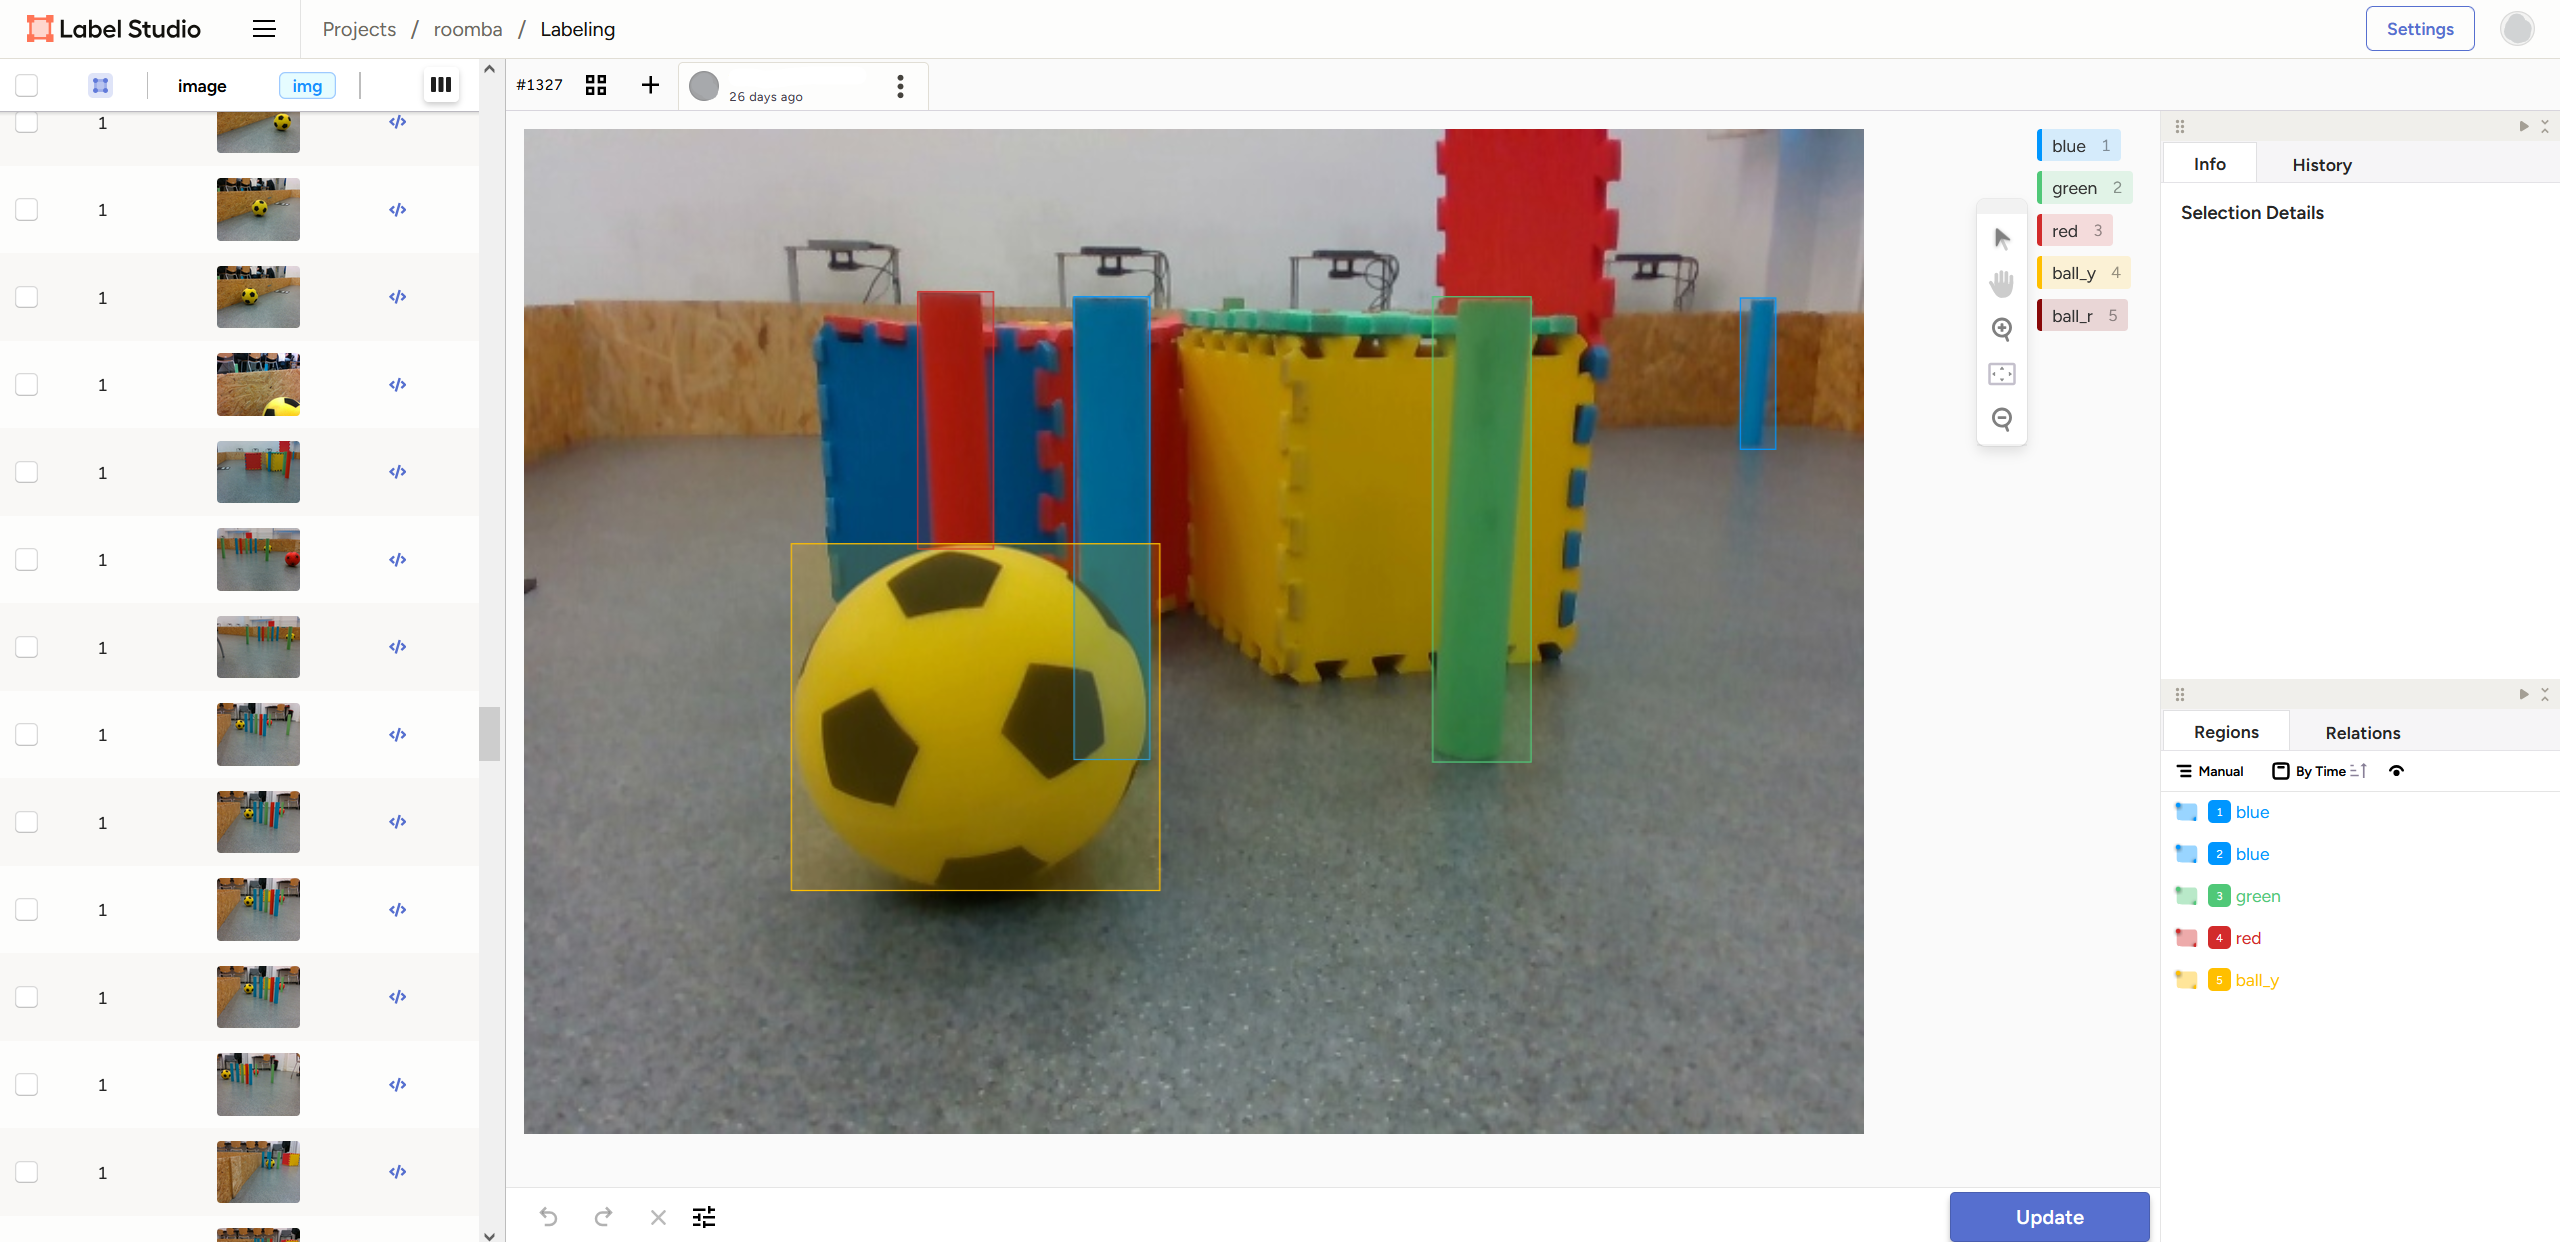
\includegraphics[width=0.8\textwidth]{pictures/label_studio.png}
    \caption{Anotování v Label Studiu}
    \label{fig:label_studio}	
\end{figure}
Pro anotaci jsme použili nastavení \textit{Object Detection with Bounding Boxes}, tedy jsme anotavali pomocí obdelníků. Zvolili jsme možnost bez rotace, všechny obdelníky mají tedy rovnoběžné strany se stranami obrazu. 
Toto představilo problém, který jde vidět v obrázku \eqref{fig:detected_image}. Díky zakřivení obrazu z kamery, obdelníky nesedí přímo na pilíře, což byl lehce vyřešitelný problém \eqref{sec:point_cloud}. Možnost segmentace, myšleno maskou jsme zamítli z různých důvodou, např. pracné anotace. 
Anotovaný data set byl poté vyexportován ve formátu YOLO.
Pomocí Python kódu a knihovny od \href{https://docs.ultralytics.com/}{Ultralitics} jsme natrénovali model. Vyzkoušeli jsme YOLO verze v8 a 11. Ukázalo se, že verze 11 je mnohem přesnější, zvláště při změně osvětlení. 
Protože detekce musí probíhat rychle, zkoušeli jsme modeli 11s a 11n. I když je model 11s přesnější, používáme ho jen výjimečně, protože může způsobit problémy pro SLAM svojí dlouhou časovou náročností. 
I pro model 11n jsme zkoušeli různé rozlišení. Rozlišení 160p a 240p bylo zpracováno dostatečně rychle a s uspokojivími výsledky. Oba modely byly natrénovany na 300 epochách.

\begin{figure}[H]
    \centering
    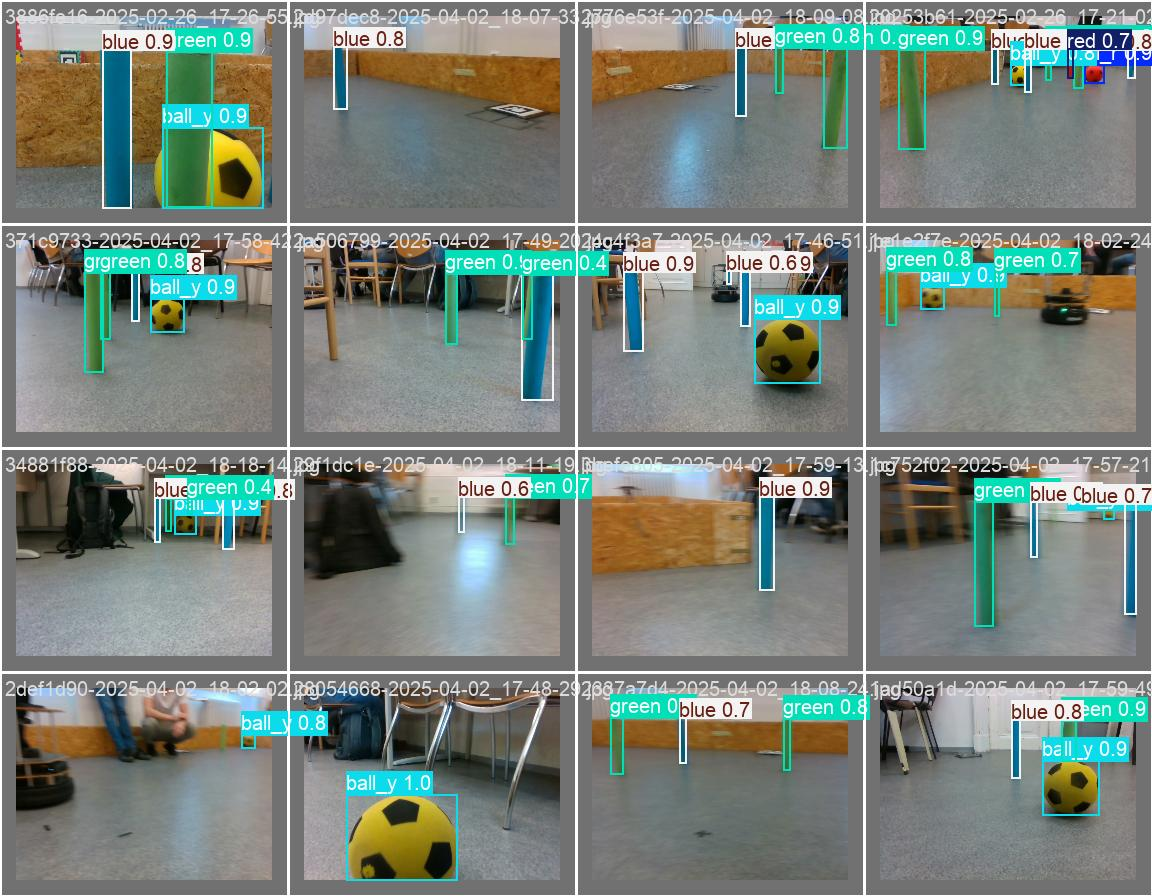
\includegraphics[width=0.7\textwidth]{pictures/rozpoznane.jpg}
    \caption{Rozpoznané objekty pomocí YO
    LO 11n při rozlišení 240p}
    \label{fig:detected_image}
\end{figure}

\begin{figure}[H]
    \centering
    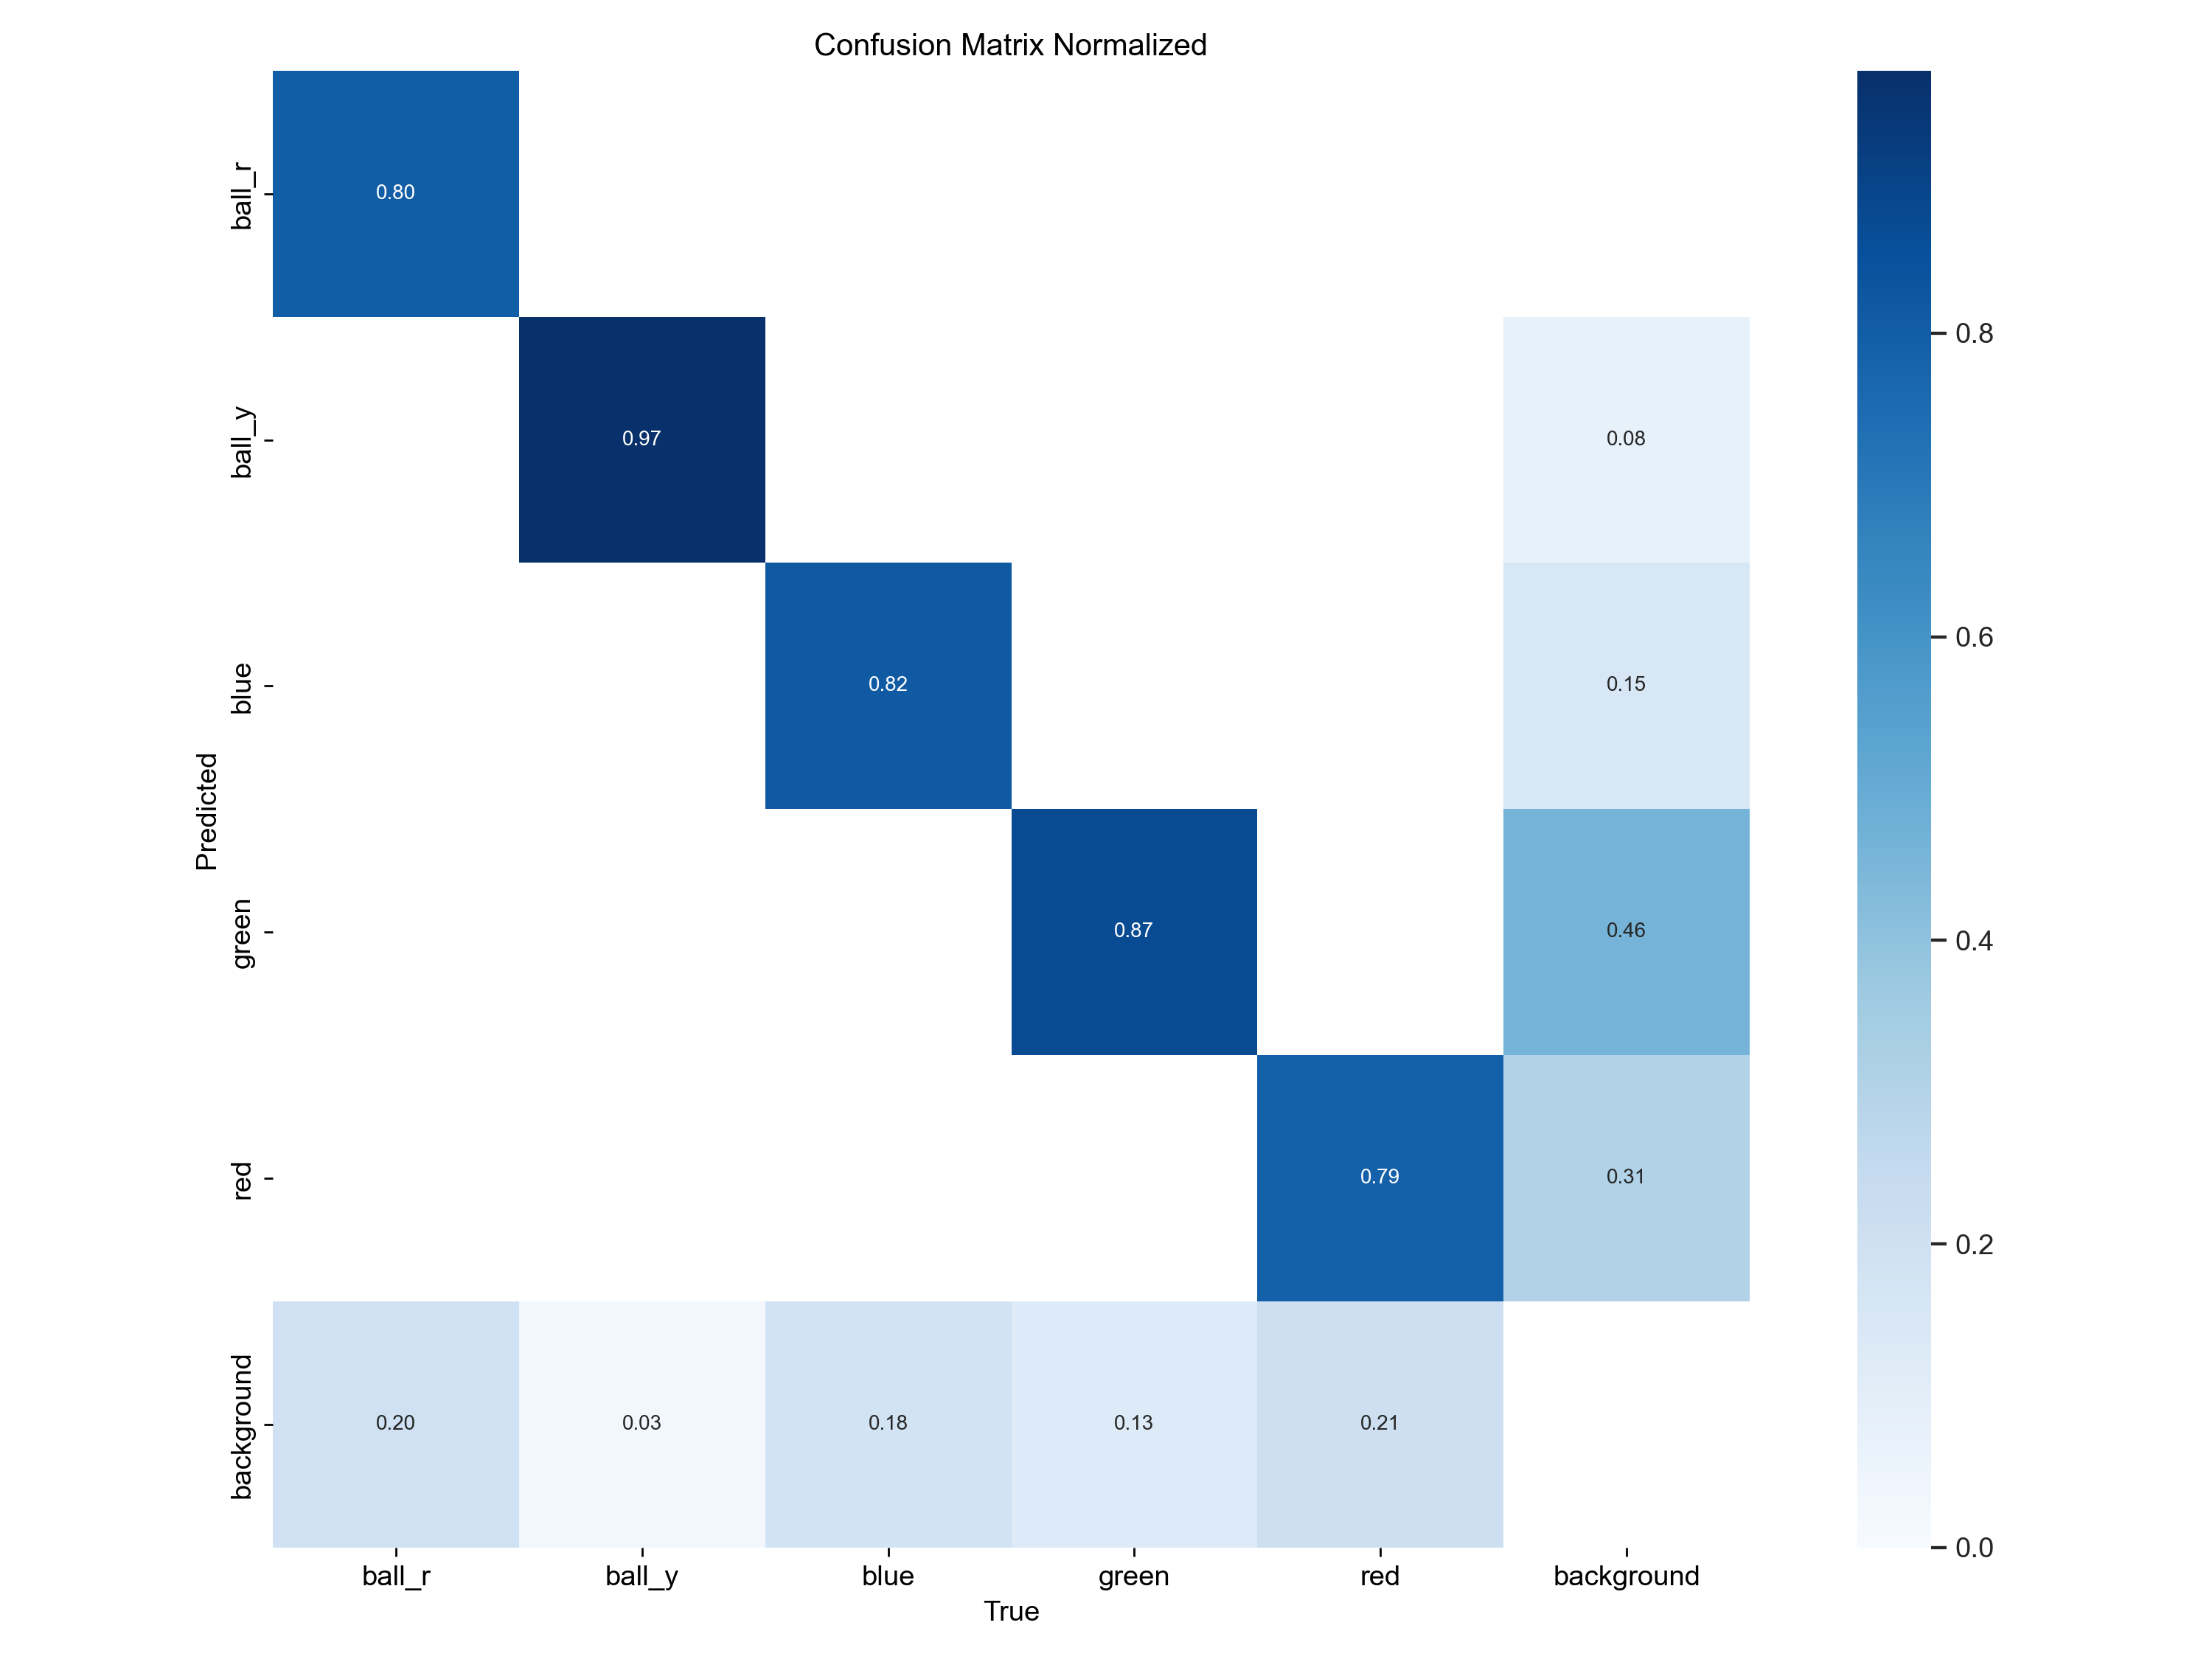
\includegraphics[width=0.8\textwidth]{pictures/v11n_160p.png}
    \caption{Normalizovaná matice záměn pro model 11n 160p}
    \label{fig:confusion_matrix_160p}
\end{figure}

\begin{figure}[H]
    \centering
    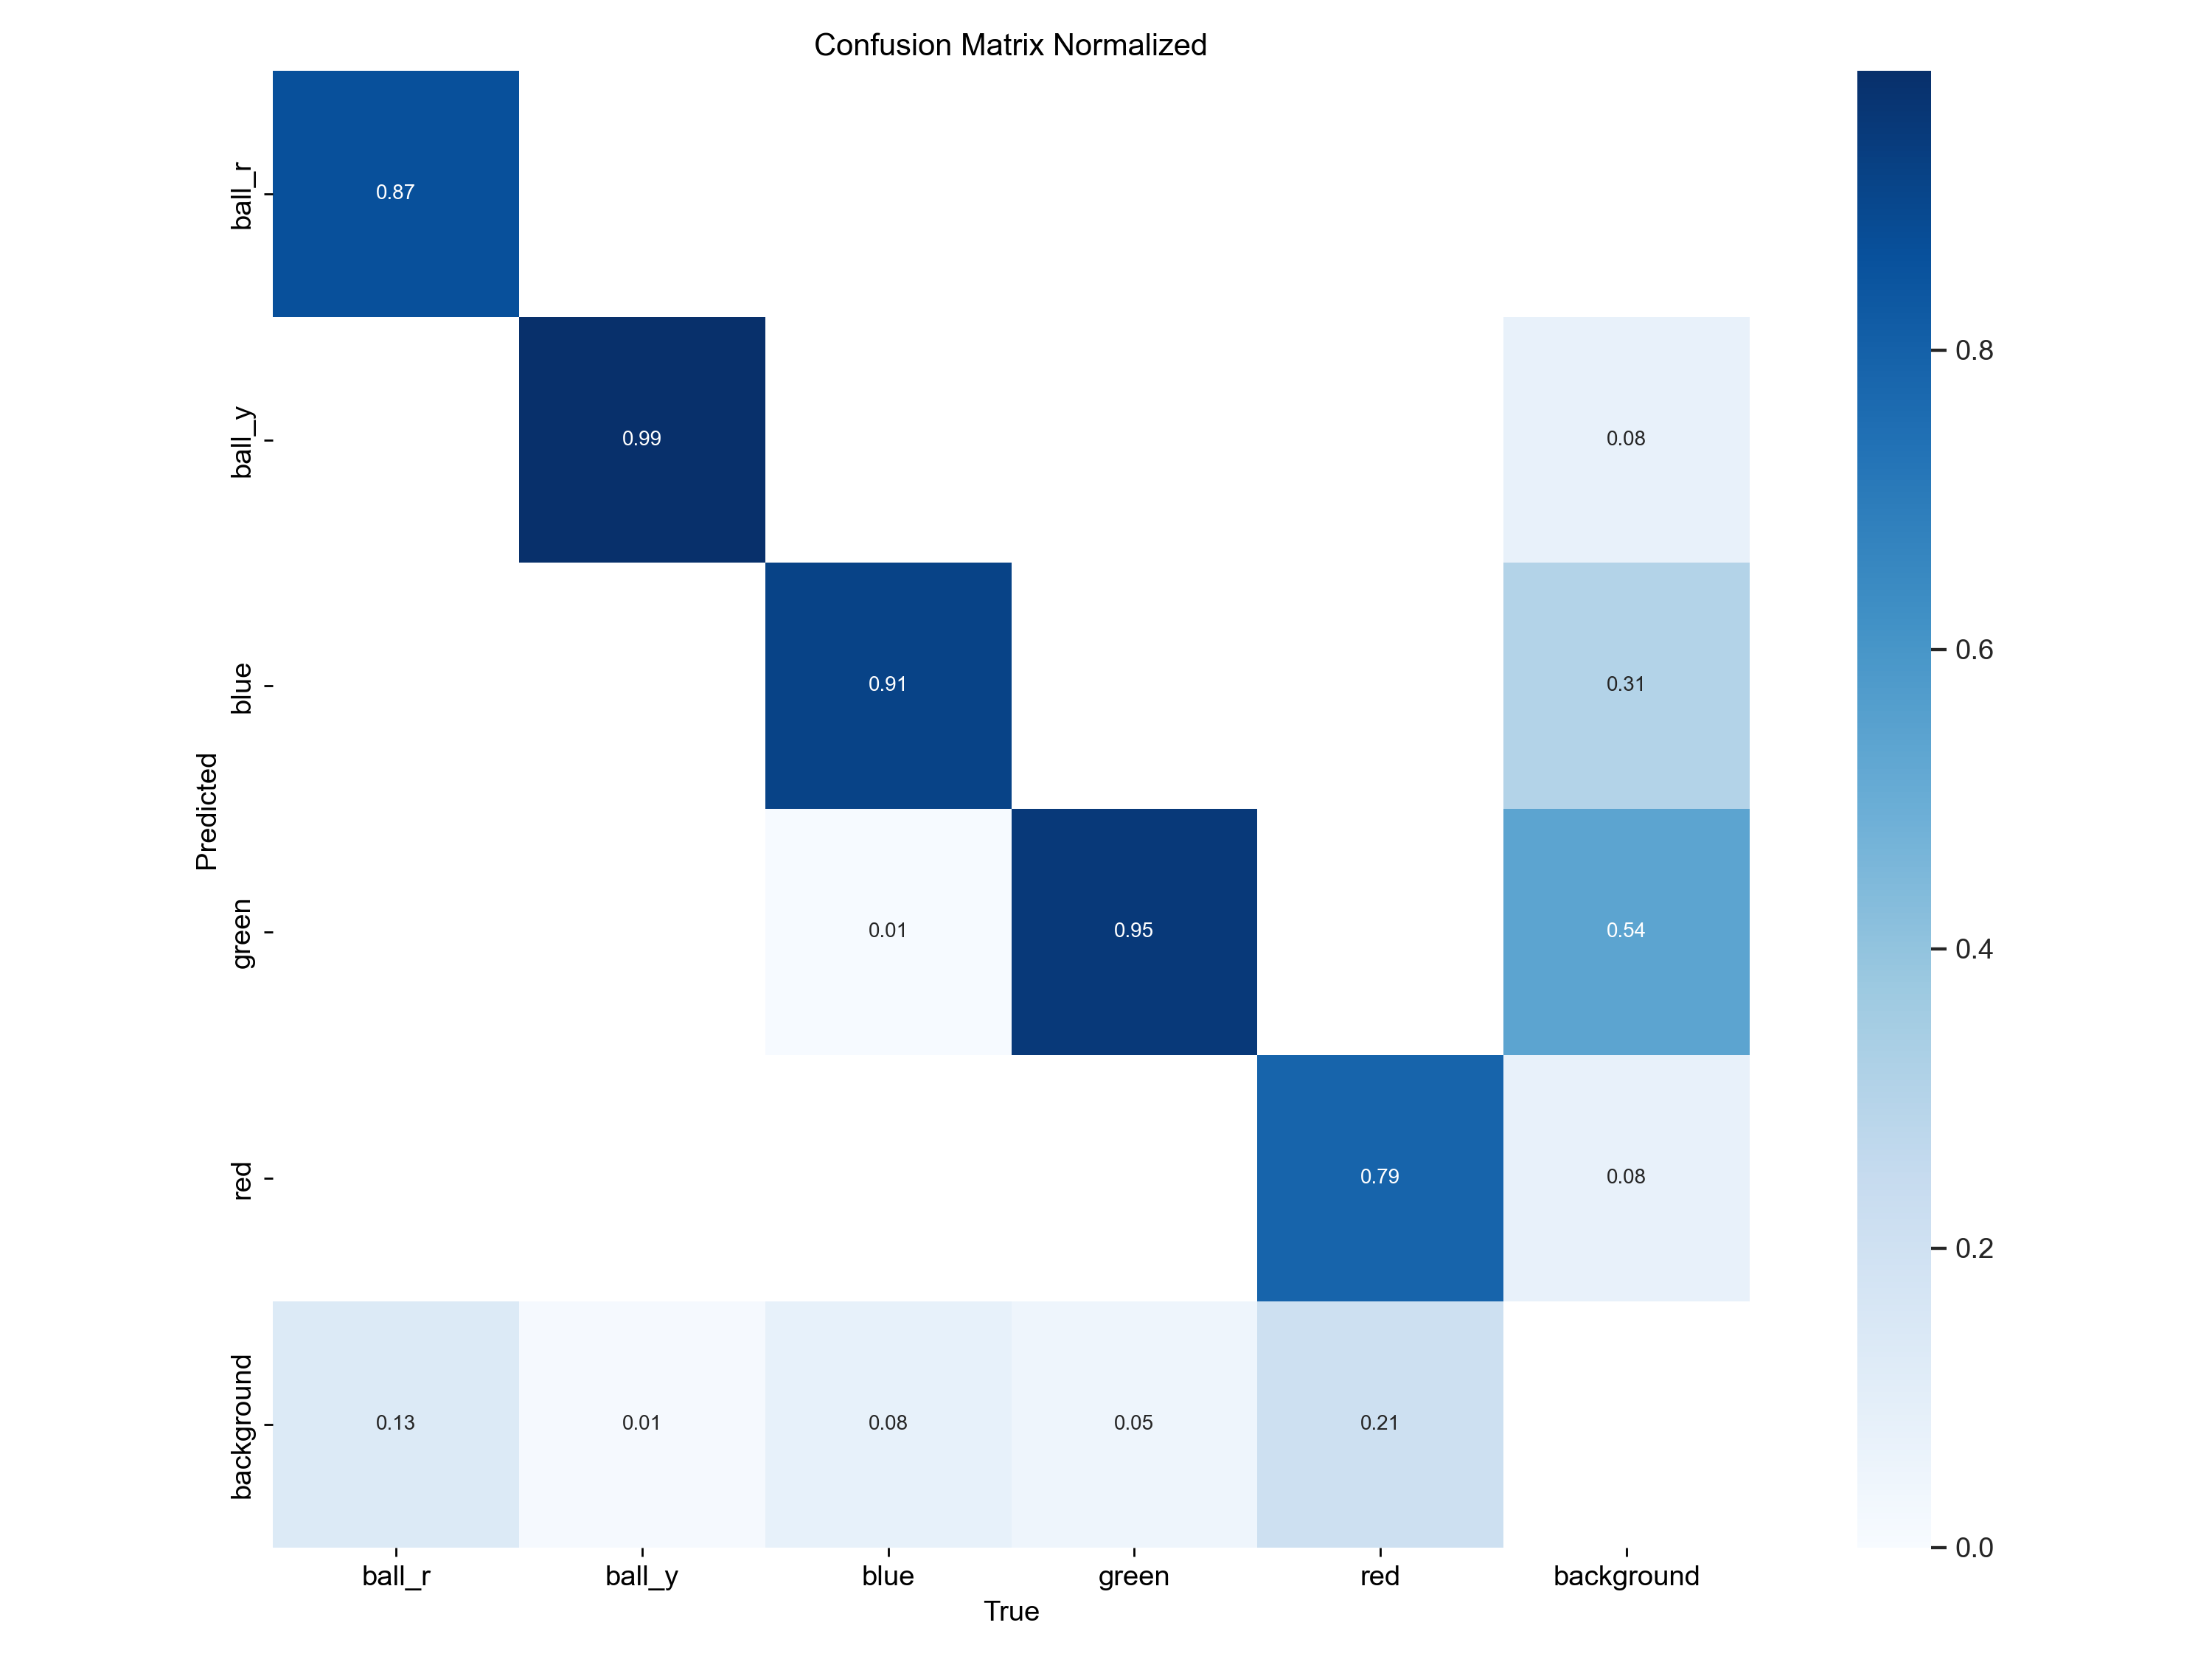
\includegraphics[width=0.8\textwidth]{pictures/v11n_240p.png}
    \caption{Normalizovaná matice záměn pro model 11n 240p}
    \label{fig:confusion_matrix_240p}
\end{figure}

Model 160p (Obrázek \eqref{fig:confusion_matrix_160p}) je v některých podmínkách znatelně horší oproti 240p (Obrázek \eqref{fig:confusion_matrix_240p}) v rozpoznávání modrých pilířů.
To může způsobit velké problémy, protože modré pilíře tvoří branku. Nejčastějším objektem, který byl zaměněn s pozadím, je zelený pilíř, který, když je detekován navíc, minimálně překaží úspěšnému vyřešení problému.
V obrázku \eqref{fig:detected_image} si ještě můžeme všimnout, že model dobře zvládá rozpoznávání objektů, které mají zaměnitelné barvy nebo tvar s objekty, které detekuje.
Model také například rozpoznal míč, když je z části za pilířem, nebo objekty, když jsou ve stínu pod stolem.

\subsubsection{Rozpoznávání obrazu}
K rozpoznávání použiváme buď model YOLO 11n při rozlišení 160p nebo při 240p v závislosti na prostředí a pokud více benefitujeme z rychlejší detekce nebo její přesnosti.
Na robotovi zajišťuje rozpoznávání class \texttt{Camera}. Třída má metodu \texttt{get detections}, která získá obraz z kamery. 
Seznam objektů vracíme pro potřeby SLAM jako numpy array poloha x, poloha y, objekt. Poloha x, y je poloha relativně k robotovi v prostoru.

K detekci nepoužíváme samotnou knihovnu YOLO. Model nejdříve konvertujeme do ONXX (Open Neural Network Exchange). Důvodem pro toto rozhodnutí je dlouhá doba, kdy YOLO knihovna zpracovála obraz. ONNX to zvládá rychleji z části díky tomu, že je optimalizovaná pro spouštění na procesoru.
Používání ONNX ale přineslo spoustu výzev, protože YOLO knihovna řešila spoustu věci za nás. Museli jsme naimplementovat počítaní pravděpodobností detekce pomocí softmax. 
Poté pomocí Non-Maximum Suppression z knihovny TorchVision řešíme odstranění duplicitních detekcí. A samozřejmostí je nepracování s detekcemi, které nedosahují nějaké hranice jistoty.

\subsubsection{Pozice objektů v prostoru}
\label{sec:point_cloud}
Z počátku jsme využívali k určování pozice objektů point cloud, který jsme získali z kamery.
To se ukázalo jako velice časově náročné. Proto jsme se rozhodli, že budeme počítat pozici objektů přímo z hloubkové kamery.
\begin{figure}[H]
    \centering
    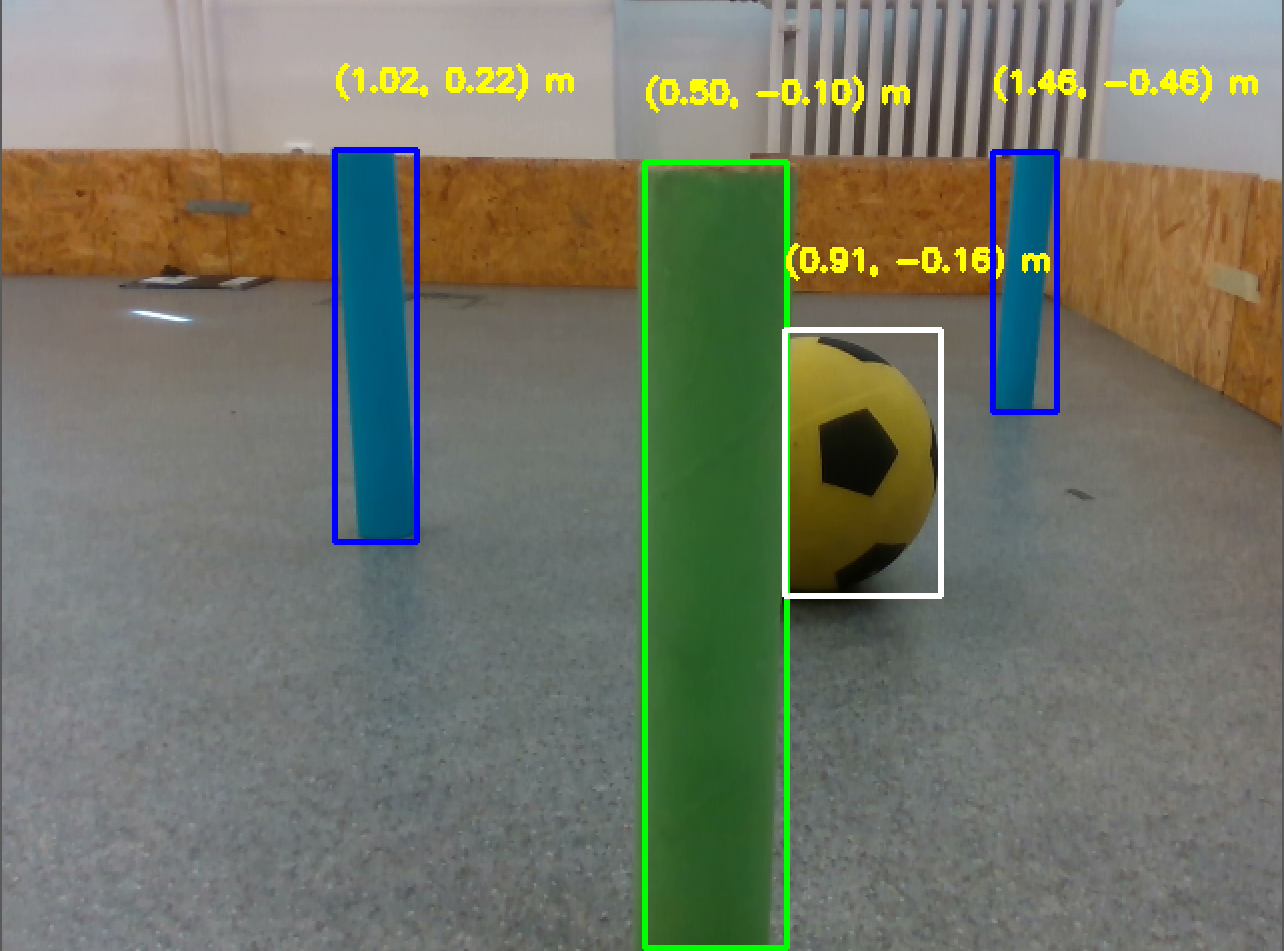
\includegraphics[width=0.5\textwidth]{pictures/detect.png}
    \caption{Obrázek z RGB kamery s rozpoznanými objekty}
    \label{fig:detect}
\end{figure}
\begin{figure}[H]
    \centering
    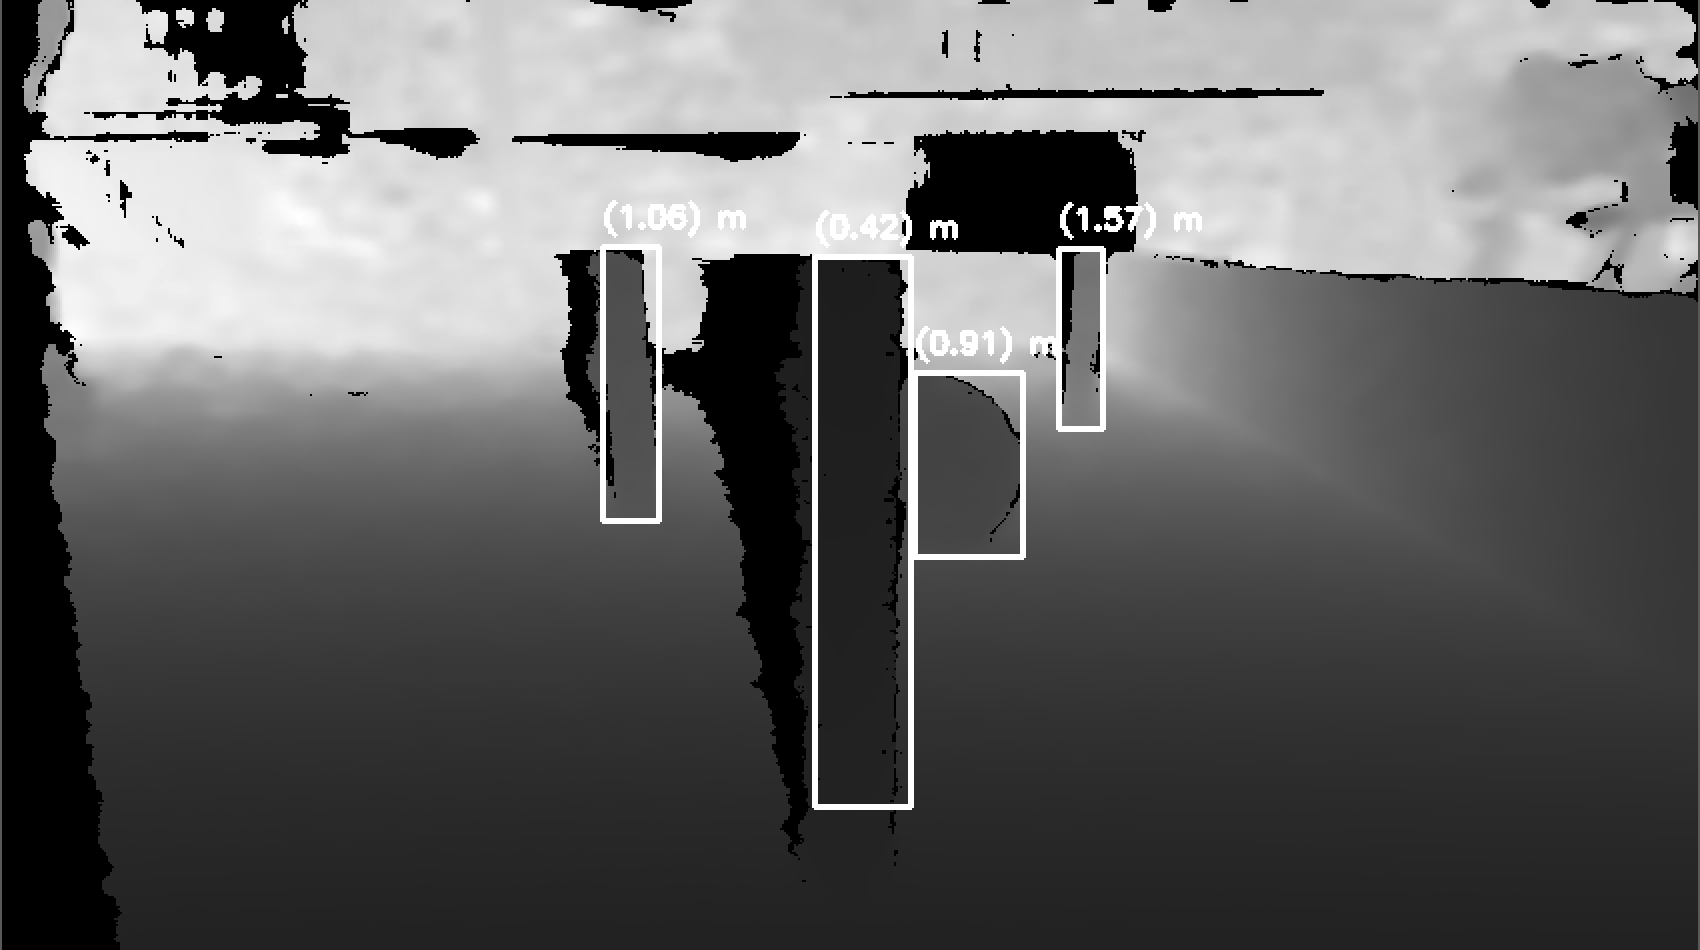
\includegraphics[width=0.7\textwidth]{pictures/depth_detect.png}
    \caption{Obrázek z hloubkové kamery s rozpoznanými objekty}
    \label{fig:depth_detect}
\end{figure}
Hloubková kamera vrací pouze pixeli s hloubkou. Aby byla poloha objektů spočítána co nejrychleji, pracujeme pouze s pixeli z hloubkové kamery (Obrázek \eqref{fig:depth_detect}), které jsou detekovány jako objekty z RGB kamery (Obrázek \eqref{fig:detect}).
Nejdříve vytvoříme transformační matici, která převadí mezi souřadnicemi kamery a hloubkové kamery. Poté se vypočítá median vzdáleností v bounding boxu, což řeší problém s obdelníky přesně nepasujícími na detekované objekty. 
Medián vzdálenosti přenásobíme konstantou 1.04, abychom korigovali nepřesnost depth kamery.
Pomocí K matice převedeme souřadnice z pixelů na reálné souřadnice vůči robotovi. Za souřadnice detekce se také přidá třída objektu.



\subsection{Lokalizace a mapování}
Jelikož je plocha, po které se pohybujeme rovná, je možné používat pouze 2D souřadnice. Pro lokalizaci robota a mapování používáme SLAM algoritmus z rodiny 
Kalman filtrů, kvůli nelinearitě transformace z globálních souřadnic do lokálních bylo potřeba použít Kalman filtr, který si umí s nelinearitami poradit. 
Tedy se nabízí dvě možnosti, Extended Kalman Filter (EKF) a Unscented Kalman Filter (UKF). Pro náš účel jsme zvolili UKF, který je přesnější a při malém počtu landmarků není výpočetně náročný.
\subsubsection{Unscented Kalman filter}
\label{sec:ukf}
Unscented Kalman Filter je založen na Unscented transformaci, která pomocí sigma bodů aproximuje nové normální rozdělení po transformaci. 
Sigma podle vzorce:
\begin{equation}
    \chi_{i} = \begin{cases}
        \mathbf{\bar{x}} & i = 0 \\
        \mathbf{\bar{x}} + (\sqrt{(n + \lambda) \mathbf P})_{i-1} & 1 \leq i \leq n \\
        \mathbf{\bar{x}} - (\sqrt{(n + \lambda) \mathbf P})_{i-1} & n + 1 \leq i \leq 2n
    \end{cases}
\end{equation}
kde $\mathbf{\bar{x}}$ je odhad střední hodnoty, $\mathbf P$ je kovarianční matice a $\lambda$ je parametr, který určuje rozptyl sigma bodů a vypočítá se podle
\begin{equation}
    \lambda = \alpha^2(n + \kappa) - n
\end{equation}
kde $\alpha$ a $\kappa = 3 - n$ jsou vstupní parametry určující rozptyl sigma a $n$ je dimenze stavového vektoru kalman filtru. 
Pro výpočet Unscented transformace jsou poutřeba ještě váhy jednotlivých sigma bodů. 
Výpočet váhy aktuální střední hodnoty pro odhad nové je dělán podle: 
\begin{equation}
    w^{m}_0 = \frac{\lambda}{n + \lambda}
\end{equation}
Pro ostatní body pak podle 
\begin{equation}
    w^m_i = \frac{1}{2(n+\lambda)} \;\;\; i = 1...2n
    \label{eq:mean_weights}
\end{equation}
Výpočet váhy aktuální střední hodnoty pro odhad nové kovarianční matice je prováděn podle vzorce
\begin{equation}
   w^c_0 = \frac{\lambda}{n + \lambda} + 1 - \alpha^2 + \beta
\end{equation}
váhy pro ostatní body pak stejně jako pro odhad střední hodnoty, tedy podle (\ref{eq:mean_weights})
\\
Po vytvoření sigma bodů a jejich vah, je možné pomocí Unscented transformace určit nový odhad střední hodnoty a kovarianční matice pro funkční hodnoty dané transformace $f$ pro všechny sigma body.
\begin{equation}
    \begin{aligned}
    \boldsymbol{\mathcal{Y}} &= f(\boldsymbol{\chi}) \\
    \mathbf{\bar{x}} &= \sum_{i=0}^{2n} w^m_i\boldsymbol{\mathcal{Y}}_i \\
    \mathbf{\bar{P}} &= \sum_{i=0}^{2n} w^c_i{(\boldsymbol{\mathcal{Y}}_i-\mu)(\boldsymbol{\mathcal{Y}}_i-\mu)^\mathsf{T}}
    \end{aligned}
    \label{eq:ukf_transform}
\end{equation}
\\
Kalman filtr má pak dva hlavní kroky, predikci a aktualizaci.\\

Predikce je provedena pomocí funkce $f$ a sigma bodů. Sigma body se transformují do nového prostoru pomocí funkce $f$ a odhadne se nová střední hodnota a kovarianční matice.
Pro UKF se pak používá Unscented transformace (\ref{eq:ukf_transform}) pro výpočet nové střední hodnoty a kovarianční matice, 
navíc je k nové kovarianční matici přičtena matice $\mathbf Q$, která je matice šumu procesu. Dostaneme tedy
\begin{equation}
    \begin{aligned}
        \boldsymbol{\mathcal Y} &= f(\boldsymbol\chi) \\
        \mathbf{\bar x} &= \sum w^m\boldsymbol{\mathcal Y}  \\
        \mathbf{\bar P} &= \sum w^c({\boldsymbol{\mathcal Y} - \mathbf{\bar x})(\boldsymbol{\mathcal Y} - \mathbf{\bar x})^\mathsf T}+\mathbf Q \\
    \end{aligned}
    \label{eq:ukf_predict}
\end{equation}

Aktualizace je prováděna pomocí měření ze senzorů, je tedy potřeba převést sigma body do prostoru měření, 
to se provádí pomocí funkce $h$ a jelikož žádné měření není přesné, tak šum měření je modelován maticí $\mathbf R$.
Pro odhad nové střední hodnoty a kovarianční matice se používá 
\begin{equation}
    \begin{aligned}
        \boldsymbol{\mathcal Z} &=  h(\boldsymbol{\mathcal{Y}}) \\
        \boldsymbol\mu_z &= \sum w^m\boldsymbol{\mathcal{Z}} \\
        \mathbf y &= \mathbf z - \boldsymbol\mu_z \\
        \mathbf P_z &= \sum w^c{(\boldsymbol{\mathcal Z}-\boldsymbol\mu_z)(\boldsymbol{\mathcal{Z}}-\boldsymbol\mu_z)^\mathsf{T}} + \mathbf R \\ 
        \mathbf K &= \left[\sum w^c(\boldsymbol{\mathcal Y}-\bar{\mathbf x})(\boldsymbol{\mathcal{Z}}-\boldsymbol\mu_z)^\mathsf{T}\right] \mathbf P_z^{-1} \\
        \mathbf x &= \mathbf{\bar x} + \mathbf{Ky}\\
        \mathbf P &= \bar{\mathbf P} - \mathbf{KP_z}\mathbf{K}^\mathsf{T}
    \end{aligned}
\end{equation}

\subsubsection{SLAM struktura}
Stavový vektor ve SLAMu obsahuje pozici robota a pozice landmarků, které robot vidí, tedy 
\begin{equation}
    \mathbf x = \begin{bmatrix}
        x \\
        y \\
        \theta \\
        x_1 \\
        y_1 \\
        x_2 \\
        y_2 \\
        \vdots \\
        x_n \\
        y_n 
    \end{bmatrix}
\end{equation}
kde $(x,y, \theta)$ je pozice robota a $(x_i,y_i)$ je pozice $i$-tého landmarku.
Jelikož máme více typů landmarků, které se liší svojí třídou, je potřeba mít pro každý landmark uloženou třídu mimo stavový vektor, 
jelikož jejich chování na ní není závislé a zbytečně by se zvedala dimenze stavového vektoru.

\subsubsection{Predikce Kalman filtru ve SLAMu}
Predikce může být provedena podle fyzikálního modelu robota v závislosti na kontolních vstupech $\mathbf u$, to je však v našem případě zbytečné,
jelikož robot nabízí odometrii, která může model nahradit. Jelikož polohy landmarků se nemění v čase, mění se pouze poloha robota. Dostaneme tedy
\begin{equation}
    f(\mathbf x,\mathbf u) = \mathbf x + \begin{bmatrix}
                                    \Delta x \\
                                    \Delta y \\
                                    \Delta \theta \\
                                    0 \\
                                    0 \\
                                    \vdots \\
                                    0
                                \end{bmatrix}
\end{equation}
Abychom zíkali pouze rozdíly z odometrie bez restartování integrace v robotovi v každé iteraci, musíme si uchovávat poslední odometrické hodnoty, označení $n-1$, a počítat rozdíly mezi nimi.
V lokálních souřadnicích robota pak dostaneme 
\begin{equation}
    \begin{bmatrix}
        \Delta x_l \\
        \Delta y_l \\
        \Delta \theta_l \\
    \end{bmatrix} = 
    \begin{bmatrix}
        (x_{n} - x_{n-1})\cos(-\theta_{n}) + (y_{n} - y_{n-1})\sin(-\theta_{n}) \\
         -(x_{n} - x_{n-1})\sin(-\theta_{n}) + (y_{n} - y_{n-1})\cos(-\theta_{n})\\
        \theta_{n} - \theta_{n-1} \\
    \end{bmatrix}
\end{equation}
Poté je potřeba převést delty do globálních souřadnic, což je v tomoto případě další rotace
\begin{equation}
    \begin{bmatrix}
        \Delta x \\
        \Delta y \\
        \Delta \theta \\
    \end{bmatrix} = 
    \begin{bmatrix}
        \Delta x_l \cos(\theta) + \Delta y_l \sin(\theta) \\
         -\Delta x_l \sin(\theta) + \Delta y_l \cos(\theta)\\
         \Delta \theta_l \\
    \end{bmatrix}
\end{equation}
Nepřesnot odometrie je modelována maticí $\mathbf Q$, která má dimenzi stejnou jako stavový vektor, bude tedy z velké části nulová. Známe pouze odchylky pro jednotlivé proměnné, které jsou v našem případě $x$, $y$ a $\theta$, tedy

\begin{equation}
    \mathbf Q_c = \begin{bmatrix}
        \sigma_{x} & 0 & 0 & 0 & ... & 0\\
        0 & \sigma_{y} & 0 & 0 & ... & 0 \\
        0 & 0 & \sigma_{\theta} & 0 & ... & 0\\
        0 & 0 & 0 & 0 & ... & 0\\
        \vdots & \vdots & \vdots & \vdots & \ddots & \vdots \\
        0 & 0 & 0 & 0 & ... & 0\\
    \end{bmatrix}
\end{equation}
to však neodpovídá transformaci, která je prováděna, tedy je potřeba použít Jacobian pro transformaci
\begin{equation}
    \mathbf J = \begin{bmatrix}
        \frac{\partial x}{\partial x_l} & \frac{\partial x}{\partial y_l} & \frac{\partial x}{\partial \theta_l} & 0 & ... & 0\\
        \frac{\partial y}{\partial x_l} & \frac{\partial y}{\partial y_l} & \frac{\partial y}{\partial \theta_l} & 0 & ... & 0\\
        \frac{\partial \theta}{\partial x_l} & \frac{\partial \theta}{\partial y_l} & \frac{\partial \theta}{\partial \theta_l} & 0 & ... & 0\\
        0 & 0 & 0 & 0 & ... & 0\\
        \vdots & \vdots & \vdots & \vdots & \ddots & \vdots \\
        0 & 0 & 0 & 0 & ... & 0\\
    \end{bmatrix} = \begin{bmatrix}
        \cos(\theta) & \sin(\theta) & 0 & 0 & ... & 0\\
        -\sin(\theta) & \cos(\theta) & 0 & 0 & ... & 0\\
        0 & 0 & 1 & 0 & ... & 0\\
        0 & 0 & 0 & 0 & ... & 0\\
        \vdots & \vdots & \vdots & \vdots & \ddots & \vdots \\
        0 & 0 & 0 & 0 & ... & 0\\
    \end{bmatrix}
\end{equation}
Výsledná matice $ \mathbf Q$ pro predikci je tedy
\begin{equation}
    \mathbf Q = \mathbf J \cdot \mathbf Q_c \cdot \mathbf J^T
\end{equation}

\subsubsection{Aktualizace Kalman filtru ve SLAMu}
Pro krok aktualizace používáme detekce z kamery, které jsou statické, to znamená, že pouze sloupky. 
Ty jsou na vstupu do SLAMu v lokálních souřadnicích robota, a mají tvar $(x_l, y_l, třída)$, kde třída je barva sloupku.
Pro vytváření mapy a lokalizaci robota však poutřebujeme souřadnice v globálních souřadnicích, pro převod do globálních souřadnic použijeme
\begin{equation}
    \begin{bmatrix}
        x_g \\
        y_g \\
    \end{bmatrix} = 
    \begin{bmatrix}
        x_r + x_l \cos(\theta) - y_l \sin(\theta) \\
        y_r + x_l \sin(\theta) + y_l \cos(\theta) \\
    \end{bmatrix}
    \label{eq:local_to_global}
\end{equation}
kde $(x_r,y_r)$ je pozice robota, $(x_l,y_l)$ je pozice landmarku v lokálních souřadnicích a $\theta$ je úhel robota. \\
V Kalman filtru však musíme transformovat souřadnice landmarků z lokálních do globálních souřadnic, to se provádí pomocí 
\begin{equation}
    \begin{bmatrix}
        x_l \\
        y_l \\
    \end{bmatrix} =
    \begin{bmatrix}
        (x_g - x_r) \cos(\theta) + (y_g - y_r) \sin(\theta) \\
        - (x_g - x_r) \sin(\theta) + (y_g - y_r) \cos(\theta) \\
    \end{bmatrix}
    \label{eq:global_to_local}
\end{equation}

Nejdůležitějším krokem v aktualizaci z landmarků z kamery je správná asociace landmarků z kamery a landmarků v mapě. 
To provádíme pomocí eukleidovské vzdálenosti mezi landmarky z kamery a landmarky v mapě.
Pokud jsou splněny podmínky v (\ref{eq:association}) pro daný landmark z kamery $L^c_i$ a landmark z mapy $L^m_j$, pak je asociace provedena podle vzorce
\begin{equation}
    min_{j} \|L^c_{i} - L^m_{j} \| = min_{k} \|L^c_{k} - L^m_{argmin_{j} \|L^c_{i} - L^m_{j} \|}\| < \epsilon
    \label{eq:association} 
\end{equation}
kde $\epsilon$ je prahová hodnota pro vzdálenost mezi landmarky. 
Tím, že jsou třídy reprezentovány jako čísla, tak je možné použít k rozlišení tříd landmarků opět (\ref{eq:association}) a to tím způsobem, 
že třídy vynásobíme $10^6$ a tím přesuneme každou třídu do jiné roviny, avšak mezi landmarky stejné třídy budou vzdálenosti stejné.\\
Measurement fukce $h$ pro asociované landmarky je pouze převod landmarků z globálních do lokálních souřadnic podle (\ref{eq:global_to_local}).
\\
Measurement noise je modelováno maticí $\mathbf R$, která má stejnou dimenzi jako měření, tedy $2k$, kde $k$ je počet asociovaných landmarků.
Známe rozptyl pro jednotlivé landmarky v lokálních souřadnicích, tedy
\begin{equation}
    \mathbf R = \begin{bmatrix}
        \sigma_{x} & 0 & 0 & 0 & ... & 0\\
        0 & \sigma_{y} & 0 & 0 & ... & 0 \\
        0 & 0 & \sigma_{x} & 0 & ... & 0\\
        0 & 0 & 0 & \sigma_{y} & ... & 0\\
        \vdots & \vdots & \vdots & \vdots & \ddots & \vdots \\
        0 & 0 & 0 & 0 & ... & \sigma_{y}\\
    \end{bmatrix}
\end{equation}

\subsubsection{Aktualizace mapy}
I když nám krok aktualizace Kalman filtru aktualizuje polohy jednotlivých namapovaných landmarků a polohu robota, je potřeba ještě přidat nové landmarky do mapy.
Jelikož nechceme kvůli stabilitě Kalman filtru mazat false detekce ze stavového vektoru a kovarianční matice, 
je potřeba rozlišit landmarky, které jsou opravdové a které jsou false detekce.\\
Z předchozího kroku máme asociované landmarky z kamery, pokud se nějaký landmark nepodařilo asociovat, tak je přidán do mapy uchazečů, 
která se nepoužívá na aktualizaci polohy ani kalman filtru, detekce jsou zde uchovány po maximální dobu $t_{max}$ od své poslední detekce. 
Pokud je zde landmark kratší dobu, je asociován s novýmy detekcemi v dalších iteracích a jehé je poloha aktualizována jako vážený průměr s váhou nové detekce $w_n = \frac{1}{1 + n}$, kde $n$ je počet detekcí daného landmarku.
Pokud je daný landnark viděn více než $n_{min}$ krát, je přidán do stavového vektoru a je rozšířena kovarianční matice s inicializací na 
\[
\mathbf P_{ln} = \begin{bmatrix}
    \sigma_{x} & 0 \\
    0 & \sigma_{y} \\
\end{bmatrix}
\]
je tedy ve tvaru 
\[
\mathbf P =
\begin{bmatrix}
    \mathbf P & \mathbf 0 \\
    \mathbf 0 & \mathbf P_{ln} \\
\end{bmatrix}
\]
a landmark je odstraněn z mapy uchazečů.
Jelikož se tím změní dimenze stavového vektoru je potřeba přepočítat parametry a vstupy Unscented transformace, tedy $\kappa$ a váhy jednotlivých sigma bodů podle postupu v kapitole \ref{sec:ukf}.\\


\subsection{Plánování}
\subsection{Pohyb}
\section{Závěr}




\end{document}